\section{The Tutamen Platform}
\label{sec:tutamen}

The Tutamen Secret Storage Platform is designed to handle the storage
of arbitrary secret material from a range of applications. In this
section, we present the Tutamen architecture and our reference Tutamen
server implementations.

\subsection{Architecture}
\label{sec:tutamen:arch}

Tutamen has three discreet architectural components:

\begin{packed_desc}
\item[Access Control Servers (ACS):] The systems responsible for
  storing and enforcing secret access control requirements and for
  authenticating secret requests.
\item[Storage Servers (SS):] The systems responsible for storing
  secrets (or parts of secrets).
\item[Applications:] The systems leveraging the Tutamen platform to
  store and retrieve secrets.
\end{packed_desc}

The bulk of all Tutamen communication occurs between an application
and one or more of each type of server. Inter-server communication is
kept to a minimum to support scalability. All communication in Tutamen
takes place via TLS~\cite{dierks2008} HTTPS connections -- and in some
cases leverages mutual TLS to provide both client and server
authentication. Both access control and storage servers are designed
to be used individually or in sets. E.g. An application may store
their secret on a single storage server and delegate access control to
a single access control server, or the application may shard its
secret across multiple storage servers and delegate access control to
multiple access control servers, or any combination thereof.

\subsubsection{Access Control Servers}
\label{sec:tutamen:arch:acs}

Tutamen access control servers (ACS) are responsible for
authenticating Tutamen requests as well as storing and enforcing all
Tutamen access control requirements. Access control servers expose a
number of core data structures that reflect the manner in which they
operate. Figure~\ref{fig:tutamen:acstructs} shows these structures.

\begin{figure}[th]
  \centering
  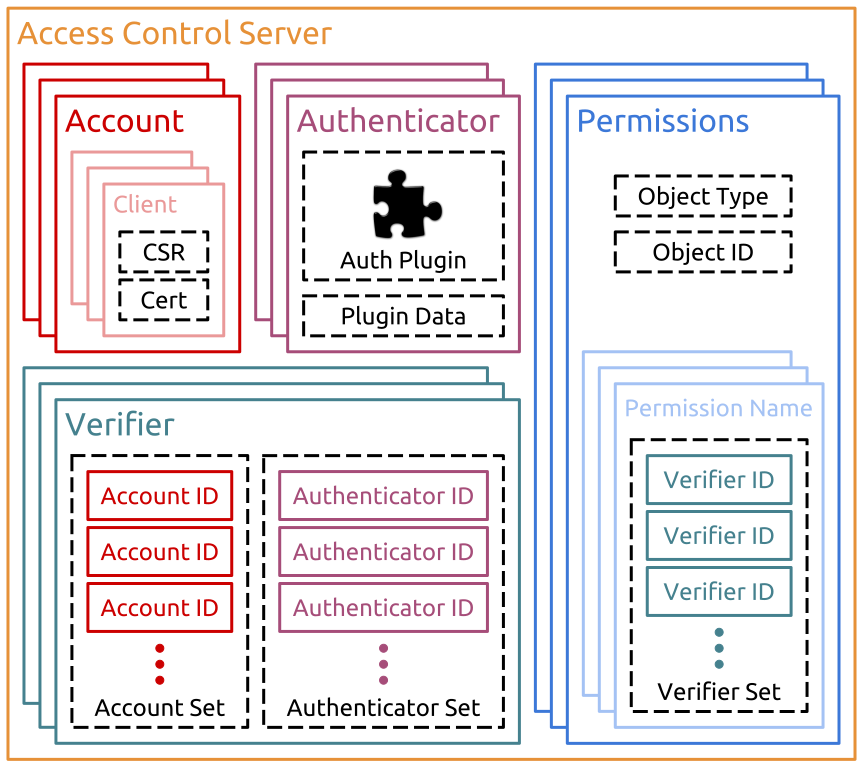
\includegraphics[width=\columnwidth]{./figs/pdf/datastructures-ac.pdf}
  \caption{Access Control Server Data Structures}
  \label{fig:tutamen:acstructs}
\end{figure}

In order to track and control access from specific actors, the access
control server uses per-actor accounts. These accounts are generally
designed to map to individual end-users, but they can be used to track
any entity to which one wishes to assign specific access control
privileges. Accounts thus form the basis of controlling and sharing
access to secrets via Tutamen. Within each account are one or more
clients. While accounts represent logically singular entities, clients
represent specific devices controlled by such entities. Each account
has one or more clients. For example, Jane Coworker may have a single
account with three clients: one for her laptop, one for her desktop,
and one for her phone.

Each client is associated with a single x509~\cite{rfc5280} TLS
key/cert-pair used to authenticate the client to the access control
server. The access control server acts as the Certificate Authority
(CA) administering these certificates. When a new client is created it
generates a local private key and uses this key to generate an X509
Certificate Signing Request (CSR). This request is then sent to the
access control server where it awaits approval from an existing client
in the account. If approved, the CSR is used to generate a signed
certificate that is sent back to the new client for use in future ACS
communication. To facilitate bootstrapping new accounts, client CSRs
are also generated and sent during new account creation. These are
atomically approved and associated with the new account -- i.e. the
initial client is created in tandem with a new account -- all
subsequent clients are then approved by previously approved clients.

In addition to accounts, the Tutamen access control server also uses
``authenticators''. Authenticators are modular mechanisms used to
implement contextual access control requirements~\cite{hulsebosch2005}
such as only allowing access during specific times of day or from
specific IP addresses. Authenticators can also be used to implement
multi-factor and/or alternate-band authentication mechanisms such as
confirming approval for a specific request from a user via text
message, or otherwise interfacing with external services to gain
approval.

Accounts and authenticators are combined via verifiers. A verifier
consists of a set of accounts and a set of authenticators. In order to
satisfy a verifier, a request must originate from a client associated
with one of the member accounts and must satisfy all of the member
authenticators. A verifier may contain no authenticators, in which
case authorization is granted solely on the basis of accounts.

The final component of the Tutamen access control server is
permissions groups. Each permissions group corresponds to a specific
object (identified via the combination of an object type and an object
ID) within the Tutamen ecosystem. A permissions groups contains one or
more permissions -- each corresponding to a specific class of actions
that can be preformed on the corresponding object. Each permission is
associated with a set of verifiers. In order to be granted a given
permission a request must satisfy at least one of the verifiers in
this set.

\subsubsection{Storage Servers}
\label{sec:tutamen:arch:ss}

Tutamen storage servers (SS) are responsible for storing all or part
of each Tutamen secret. Figure~\ref{fig:tutamen:storagestructs} shows
the core storage server data structures.

\begin{figure}[th]
  \centering
  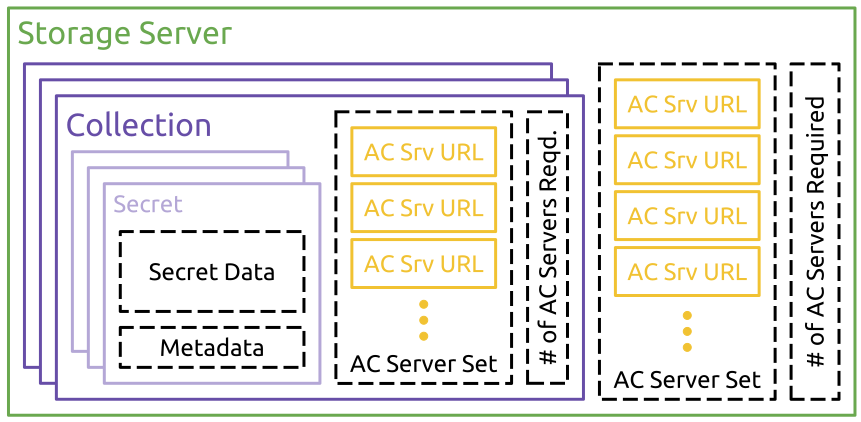
\includegraphics[width=\columnwidth]{./figs/pdf/datastructures-storage.pdf}
  \caption{Storage Server Data Structures}
  \label{fig:tutamen:storagestructs}
\end{figure}

The top-level data structure employed by storage servers is the
``collection''. A collection represents a logical grouping of one or
more secrets (or parts of secrets). Associated with each collection is
a list of one or more access control servers delegated with enforcing
the access control requirements for the collection. Access control
granularity is thus set at the per-collection, not per-secret level. A
collection is also capable of storing user-provided metadata to aid in
the mapping of collections to the objects for which they store
secrets.

Each collection stores one or more secrets or secret shards. These
secrets consist of the actual secret data the applications leveraging
Tutamen wishes to store as well as any associated user-provided
metadata. Since access control is set at the per-collection level,
secrets inherit the access control characteristics of the
corresponding collection.

How best to map secret data to collections is left up to each
application. This decision is primarily driven by the fact that access
control is preformed on the per-collection level. Thus, if an
application requires that a set of secrets always have a common set of
access control requirements (e.g. per-sector encryption keys for a
encrypted block device), it become efficient to group these secrets
into a single collection. Doing so minimizes the complexity of trying
to keep access control requirements synced across multiple secrets,
and increases performance by minimizing the number of requests that
the applications must make to secure tokens from the access control
server. In cases where each secret requires its own access control
requirements (e.g. per-file encryption keys), it is appropriate for
the corresponding application to store only a single secret per
collection.

\subsubsection{Access Control Protocol}
\label{sec:tutamen:arch:acp}

Access control servers control access related to both internal
(i.e. access control server) and external (i.e. storage server)
objects by providing signed authorization tokens in response to valid
requests. Similar to previously proposed distributed and federated
access control systems~\cite{Calero2010, Leandro2012},
each authorization token grants the bearer a specific permission
related to a specific object. Unlike previous systems, however,
Tutamen is designed to avoid needing to trust any single access
control provider (see \S~\ref{sec:tutamen:arch:distributed}).
Figure~\ref{fig:tutamen:systembase} shows the basic communication
involved in the Tutamen access control process.

\begin{figure}[th]
  \centering
  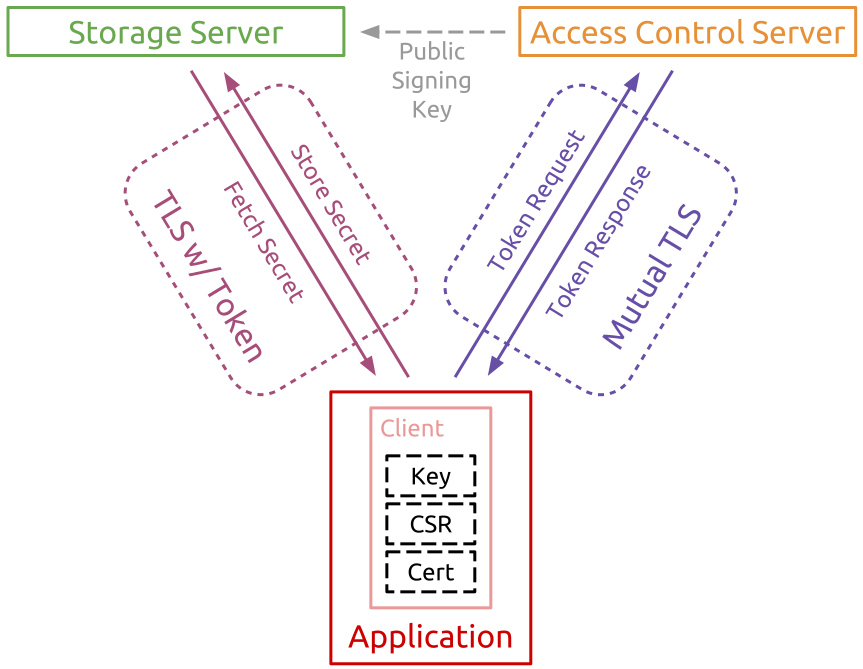
\includegraphics[width=\columnwidth]{./figs/pdf/system-base.pdf}
  \caption{Access Control Communication}
  \label{fig:tutamen:systembase}
\end{figure}

Each access control server generates authorization tokens in response
to a client sending an authorization request. Each authorization
request (and each corresponding token) includes two claims binding it
to a specific object: the object type and the object ID. Each token
request also contains a claim that binds it to a specific permission
(e.g. read, write, delete, modify) for the corresponding
object. Authorization requests are further bound to the specific
client making the request (authenticated via mutual-TLS), and to an
expiration time after which the token is no longer valid.

Upon receiving an authorization request from a client, the access
control server looks up the permission group for the corresponding
object (identified via the combination of object type and object ID)
and then loads the verifier set corresponding to the requested
permission. The server then traverses each verifier in this set --
verifying both client membership in one of the accounts listed in the
verifier as well as executing any authenticator modules required by
the verifier until it finds (or fails to find) a verifier that is
satisfied by the request. If the server is able to verify compliance
with at least one verifier it grants the authorization request and
returns a signed authorization token that includes the object type,
object ID, granted permission, and expiration time. The bearer of this
token can then present it in conjunction with a request to either the
access control server or a storage server in order to be granted the
right to perform an approved action on the corresponding object.

Other than the bootstrapping operations and the token request
operations themselves, all requests to either storage or access
control servers must be accompanied by a valid token. The receiving
server validates this token using the public signing key of the
associated AC server; for requests to the AC sever itself, this key is
available internally. For requests to external storage servers, the
signing key is downloaded by the storage server from the access
control server and cached for future use. In this manner, access
control servers are responsible both for granting and verifying
authorization requests and signing the corresponding tokens, as well
as for verifying tokens accompanying requests to preform actions on
ACS objects (e.g. to create or modify verifiers or accounts). Storage
servers are responsible only for verifying tokens accompanying
requests to perform actions on SS objects (e.g. to create a collection
or read a secret).

\subsubsection{Distributed Usage}
\label{sec:tutamen:arch:distributed}

Tutamen is designed to be used in both centralized and distributed use
cases. The simplest Tutamen arrangement (e.g. as shown in
Figure~\ref{fig:tutamen:systembase}) involves leveraging a single
Tutamen access control server and a single storage server. In this
arrangement, the storage server stores a complete copy of each secret
while the access control server is charged with solely enforcing access
to these secrets. While this use case is easy to deploy, it has two
notable downsides. First, it forces the user to place a high degree of
trust in the operator of the access control server (who has complete
control over whether or not the access control rules for a given
secret are being faithfully enforced) as well as the operator of the
storage server (who, likewise, must faithfully verify incoming tokens
and avoid otherwise leaking secret data). Second, it lacks any form of
redundancy -- if either the access control server or the storage server
is unavailable, applications will be unable to retrieve any secrets.

A variety of systems have been proposed with the goal of minimizing
trust requirements for cloud infrastructure~\cite{bessani2011,
  kallahalla2003, kubiatowicz2000, mahajan2011,
  wilcox-o'hearn2008}. Tutamen applies similar ``minimal-trust'' goals
to the secret storage problem by offering support for a distributed
operation mode as an alternative to single-server operation. Operating
Tutamen in a distributed manner is largely a task that is pushed down
to the application (or client library) -- with the exception of
offering the necessary primitives to support such operation, both
Tutamen storage and access control servers are designed to by largely
agnostic to whether they are being used in a centralized or a
distributed manner. This design has the benefit of avoiding
server-side scaling challenges, allowing the extra overhead required
for distributed operation to be supported by each application that
requires it.

\begin{figure}[th]
  \centering
  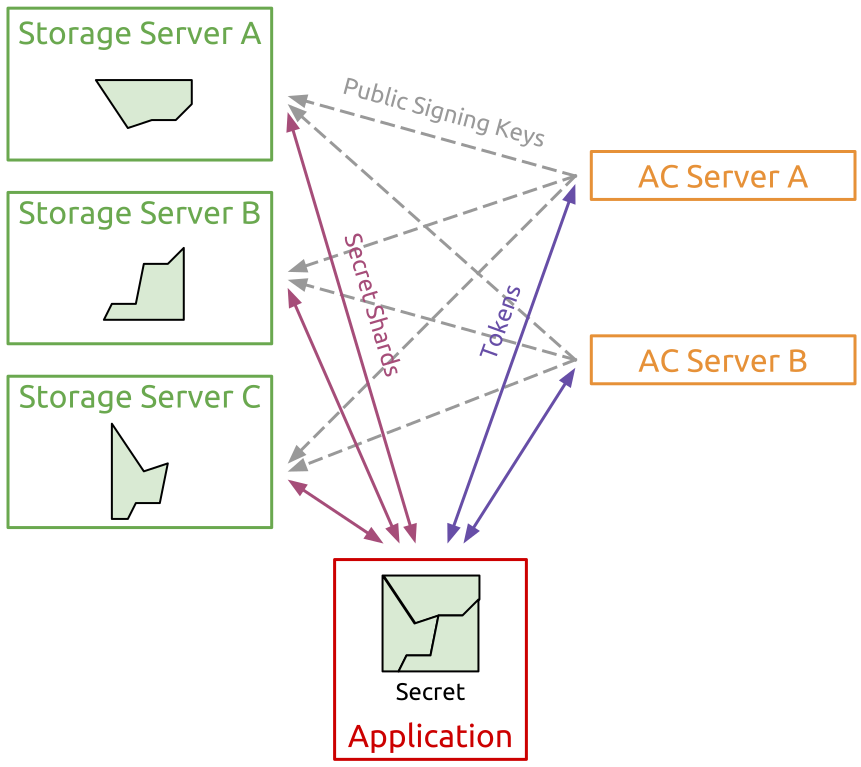
\includegraphics[width=\columnwidth]{./figs/pdf/system-distributed.pdf}
  \caption{Distributed Operation}
  \label{fig:tutamen:systemdistributed}
\end{figure}

Figure~\ref{fig:tutamen:systemdistributed} shows the basic layout of a
distributed Tutamen setup. In such a setup, the Tutamen application
first shards its secret using a $(k, n)$ threshold
scheme~\cite{shamir1979, krawczyk1993}, similar to other proposed
``minimal trust'' cloud systems~\cite{bessani2011} as well as
previously proposed ``key escrow'' systems~\cite{blaze1996,
  denning1996}. The application chooses the value of $n$ based on the
number of storage servers they wish to utilize. The value of $k$ is
then chosen to control how many of the servers must be responsive in
order to retrieve the secret -- i.e. the difference between $n$ and
$k$ controls how much storage redundancy the system has by dictating
the number of storage servers that can be unavailable before access to
the secret itself is lost. The application then pushes each shard to
the $n$ storage servers. If the application is merely concerned about
storage redundancy, or about their ability to trust a storage server
operator, it can delegate the access control for each secret shard to
a single access control server. To retrieve such a secret the
application would request the necessary token from the access control
server and include it in its request to each storage server for their
respective shard of the secret. When the application receives a
response from $k$ of the storage servers, it is able to reconstruct
the original secret.

In most cases, however, we imagine that in addition to wishing to
mitigate storage server trust and reliability failures, the
application will also wishes to protect itself against access control
server trust and reliability failures. This is accomplished via
storage server support for the specification of two pieces of access
control metadata corresponding to each stored collection: a list of AC
servers approved to provide access control tokens for the collection
and a minimum number of servers from which valid tokens must be
received. These parameters form the basis of a novel $(k, n)$
threshold scheme for access control servers -- e.g. a collection may
delegate a list of $n$ access control servers from which an
application must acquire at least $k$ valid tokens in order to gain
access. Thus, if the user does not wish to trust a single access
control server, they may require tokens from at least $k$ different AC
servers in order to access the data stored in a given
collection. Likewise, if the application wishes to withstand the
failure of one or more AC servers, it can specify $n$ possible AC
servers where $n > k$.

In order to facilitate ease of management when operating in a
distributed mode, Tutamen also supports allowing applications to
request specific UUIDs~\cite{leach2005} for each object at creation.
This allows clients to use the same object ID across multiple servers,
alleviating the burden of maintaining a mapping between object IDs and
the servers to which they correspond. Using the same object IDs across
multiple servers also allows for more efficient token management --
e.g if an application uses the same collection ID on three separate
storage serves, all of which delegate a common set of access control
servers, it's possible (and desirable) for the application to use a
single token granting access to the relevant collection ID on all
three servers. Without this capability, an application would be forced
to request multiple tokens from each access control server
corresponding to the collection ID used on each storage
server.\footnote{The ability to request specific object IDs does have
  one downside -- it opens Tutamen up to a possible denial-of-service
  (DoS) attack where an attacker attempts to request the object IDs
  they know another application wishes to use for themselves. Since
  each server may only use each object ID once, the first application
  to request a given UUID gets it. Thus, if an adversary knew which
  object IDs a given application planned to use, they could request
  these object IDs on a set of AC servers for themselves, depriving
  the original application of the ability to use those servers. None
  the less, we believe the convenience afforded by allowing
  applications to request specific object IDs outweighs the potential
  for DoS abuse.}

\subsection{Implementation}

In order to demonstrate and test the Tutamen platform we've created
reference implementations for the storage server, access control
server, and several client libraries.

Our Tutamen server implementation exposes a RESTful
interface~\cite{fielding2000} for both the access control and storage
server APIs. This interface both accepts and responds using
JSON~\cite{json} messages over the HTTPS protocol. The full access
control server API specification as well as the API reference
implementation source code is available online
at~\cite{src-tutamen-apiaccesscontrol}. Likewise, the storage server
API specification and source code can be found
at~\cite{src-tutamen-apistorage}. Both implementations are freely
available under the terms of the AGPLv3. The prototype servers are
written in Python 3 using the Flask web
framework~\cite{python-flask}. For simplicity, both servers are
designed to be served via WSGI~\cite{pep3333} using the Apache HTTP
Server~\cite{apache} for TLS termination and client-certificate
verification.

Both Tutamen servers rely on a shared \texttt{pytutamen-server} python
library for the implementation of their core logic. The
\texttt{pytutamen-server} source is available
at~\cite{src-tutamen-pytutamenserver} under the terms of the
LGPLv3. This library leverages the Redis~\cite{redis} key-value store
for persistent storage. Our Tutamen implementation adopts the JSON Web
Signature (JWS)~\cite{rfc7515} and JSON Web Token (JWT)~\cite{rfc7519}
specifications for exchanging cryptographically authenticated, tokens
between Tutamen applications, access control servers, and storage
servers. We leverage the pyjwt~\cite{pyjwt} library for JWS and JWT
support. These tokens are then attached to subsequent requests using a
\texttt{tutamen-tokens} header field.

The access control servers expose a pluggable authenticator interface
through which end users and other developers may add custom
authentication functionality. This interface is similar in purpose to
previous pluggable authentication interfaces such as
PAM~\cite{samar1996}. The Tutamen authenticator interface is primarily
designed for providing authentication checks beyond the TLS
certificate based authentication the access control server
automatically performs on every request for the purpose of associating
each request with a specific client and account. As an example, we've
implemented an authenticator module that allows users to approve
Tutamen token requests via SMS text message using the
Twilio~\cite{twilio} messaging platform. We also envision
authenticator modules for enforcing access control rules such as only
allowing requests during certain times of day of from specific network
addresses. Each authenticator plugin is provided with both a set of
per-instance configuration data (i.e. to whom an SMS message gets sent
for approval) as well as all of the details of a specific token
request including both the IDs and metadata associated with the
requesting account and client (e.g. from which information such as
originating IP address or time of day can be extracted).

In addition to the server and authenticator implementations, we've
also created reference Tutamen client libraries for both
Python~\cite{src-tutamen-pytutamen} and
Go~\cite{src-tutamen-go}. Using the Python client library, we've
created a reference Tutamen CLI through which users may directly
store/retrieve secrets and control secret sharing and access control
rules. The CLI is useful for managing Tutamen objects even in cases
where other applications (e.g. those discussed in
Section~\ref{sec:apps}) are setup to interface directly with the
Tutamen platform. In this manner, it's not necessary for every Tutamen
application to implement all Tutamen functionality -- i.e. an
application might leverage only the necessary Tutamen commands to
perform secret storage and retrieval, leaving the task of managing the
sharing of Tutamen-stored secrets to the CLI or to another dedicated
management application.

\subsection{Usage Example}

To illustrate the interaction of the various components of the Tutamen
platform, we present an example of the steps taken by an application
to store and then retrieve a secret via Tutamen. In this example, we
assume the application is using three storage servers and two access
control servers as shown in
Figure~\ref{fig:tutamen:systemdistributed}. We also assume the
application has already bootstrapped an account and client -- e.g. it
previously contacted the AC servers with a request to create a new
account and associated client.

\begin{figure}[th]
  \centering
  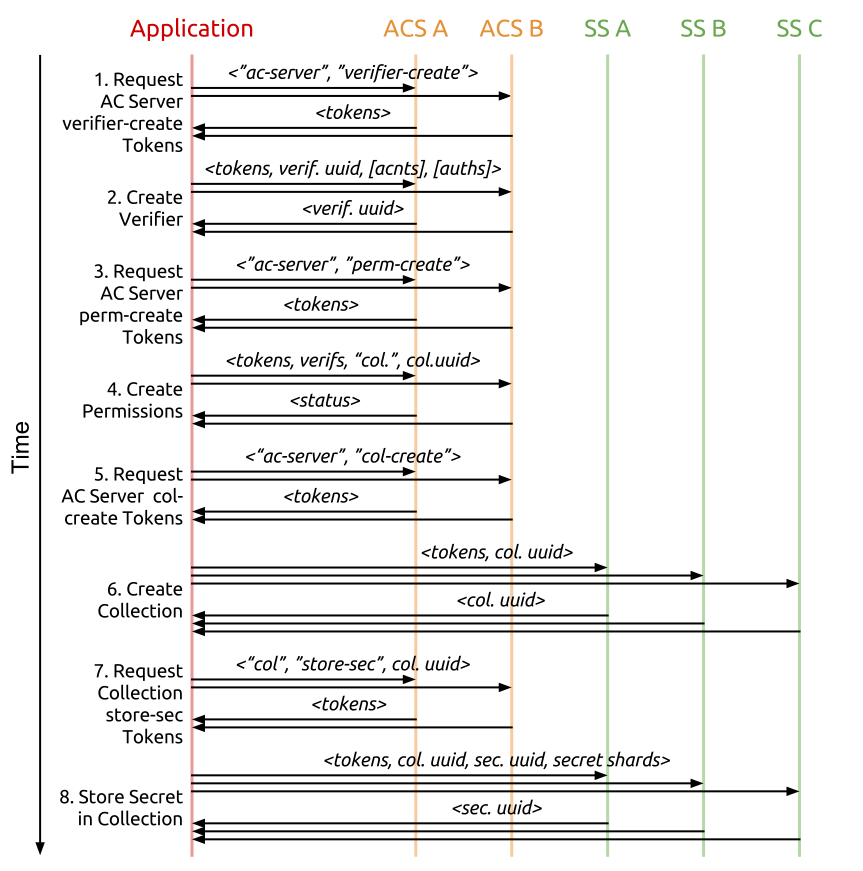
\includegraphics[width=\columnwidth]{./figs/pdf/store-secret.pdf}
  \caption{Storing a New Secret}
  \label{fig:tutamen:storesecret}
\end{figure}

Figure~\ref{fig:tutamen:storesecret} shows the steps required to store
create a new collection and store a secret within it.\footnote{Skipped
  from this diagram is the process of creating verifiers and
  permissions groups for the collection verifier itself. These
  permissions groups are necessary to control who can read, modify, or
  delete the corresponding verifier after creation. The process for
  creating said structures is similar to the process of creating the
  collection-related verifier and permissions group shown. To avoid
  the infinite recursion of needing verifiers for each verifier, it's
  possible for a verifier to be associated with a permissions group in
  which it is itself a member (e.g. a verifier can enforce its own
  access control specification).}

\begin{figure}[th]
  \centering
  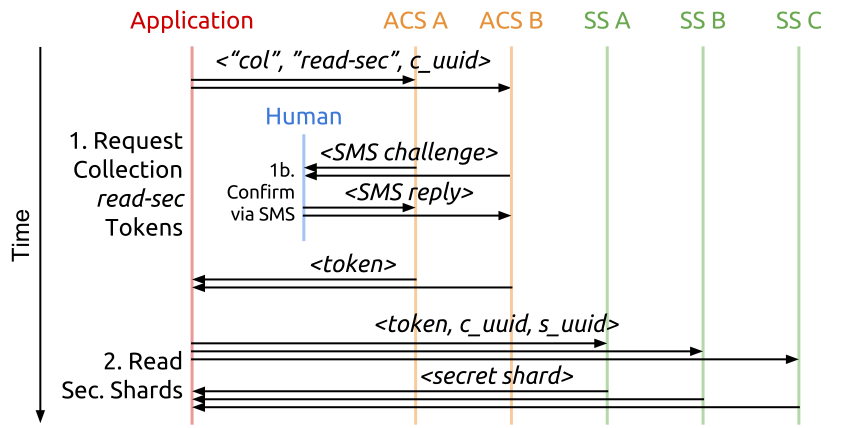
\includegraphics[width=\columnwidth]{./figs/pdf/fetch-secret.pdf}
  \caption{Retrieving an Existing Secret (w/ SMS Auth)}
  \label{fig:tutamen:fetchsecret}
\end{figure}

Figure~\ref{fig:tutamen:fetchsecret} shows the steps required to
retrieve an existing secret. This diagram also assumes that the secret
in question has an SMS authenticator associated with it -- requiring a
user to provide a response to an SMS challenge approving access to the
secret.

%%  Localwords:  Tutamen ACS HTTPS CSR CSRs Authenticators verifiers
%%  LocalWords:  authenticators authenticator
%%  LocalWords:  DoS SMS Redis AGPLv JWS JWT pyjwt pytutamen LGPLv
%%  LocalWords:  Twilio tutamen Auth
